\section{Architettura}

\begin{figure}[ht]
	\centering
	\includegraphics[width=\textwidth]{Architettura}
	\caption{Architettura del software}
	\label{fig:architecture}
\end{figure}

Il nostro software si compone di tre nodi:
\begin{itemize}
    \item Un nodo che implementa il servizio di object detection, che riceve in input un’immagine da analizzare e, per ogni oggetto nell’immagine, restituisce il relativo bounding box, la classe ed il livello di confidenza relativo alla predizione.
    \item Un nodo che implementa tre servizi che forniscono un’interfaccia verso le funzionalità di text to speech, gestione della posa e movimento della testa di Pepper.
    \item Un nodo master che implementa la funzionalità richiesta dall’homework acquisendo le immagini dal topic della camera di Pepper e utilizzando i servizi offerti dagli altri due nodi.
\end{itemize}
Per l’interfacciamento da e verso Pepper viene utilizzato il NaoQi SDK.

Qua parliamo anche del meccanismo scelto di comunicazione tra i nodi.


\subsection{Server di Object Detection}

Come anticipato, uno dei tre nodi principali del sistema si occupa di esporre un servizio di object detection. 
Questo servizio è implementato attraverso una classe chiamata \verb|PepperObjectDetectorService|, il cui diagramma UML (semplificato) è riportato in figura~\ref{fig:detector_uml}.

\begin{figure}[ht]
	\centering
	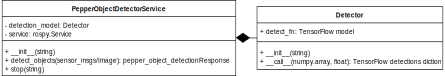
\includegraphics[width=\textwidth]{DetectorUml}
	\caption{Diagramma UML (semplificato) classe \texttt{PepperObjectDetectorService}}
	\label{fig:detector_uml}
\end{figure}

Nel costruttore della classe viene inizializzato il servizio ROS, al quale viene associato come handler il metodo \verb|detect_objects|, e viene inoltre creato un oggetto del tipo \verb|Detector|, che carica il modello di object detection dal percorso fornito e lo esegue sugli input che gli vengono sottomessi tramite chiamata. Il \verb|Detector| viene utilizzato in \verb|detect_objects| per eseguire la detection sugli input inviati al servizio.

Quando il nodo server viene eseguito, viene istanziato un oggetto del tipo 
\verb|PepperObjectDetectorService|, ed il suo metodo \verb|stop| viene registrato per l'esecuzione al momento dello shutdown del nodo, in modo tale che il servizio venga stoppato quando l'esecuzione del server termina. 
Infine il nodo entra in \verb|spin|, in modo da restare in ascolto delle richieste all'object detector.

\subsection{Server di interfaccia verso Pepper}

\subsection{Nodo Master}

Il nodo Master (come \emph{puppet master}, ossia il burattinaio) è stato concepito come il pezzo centrale della nostra applicazione. Questo nodo si interfaccia con tutti i nodi dell'architettura, ed esegue tutti i passi chiave del task in modo sequenziale. La sequenza di passi è strettamente legata al task, ed è estremamente semplice scrivere un nuovo nodo che lo sostituisca ed esegua qualsiasi altro task invocando le funzioni di interfaccia disponibili.

Abbiamo scelto l'approccio sequenziale per semplicità di implementazione. Ciò non toglie che alcune delle azioni possano ottimizzate tramite parallelismi e sincronizzazioni, ma è stato scelto di posticipare questi miglioramenti per dare precedenza al funzionamento completo del sistema secondo le specifiche.

